\documentclass[12pt,a4paper]{article}

\usepackage[T1]{fontenc}
\usepackage[utf8]{inputenc} % Use UTF-8 encoding for input
\usepackage{babel} 
\babelprovide[import=fr, main]{french} % Set the document language to French
       
\usepackage{lmodern}			       
\usepackage{amsmath}
\usepackage{amsfonts}
\usepackage{amssymb}
\usepackage{graphicx}
\usepackage{xcolor}
\usepackage{mathtools}
\usepackage{fancyhdr}
\usepackage{enumitem}
\usepackage{tcolorbox}
\usepackage{stmaryrd}
\usepackage[linesnumbered,ruled,vlined]{algorithm2e}
\usepackage[text={15cm,24.5cm},centering]{geometry}


% Définir la fonction pour créer une boîte de code
\newcommand{\code}[1]{%
    \begin{tcolorbox}[colback=black!10!white,colframe=black]
        #1
    \end{tcolorbox}
}


\begin{document}

\begin{figure}[t]
    \centering
    
\includegraphics[width=5cm]{src/inp_n7.png}
    \hfill
    
\includegraphics[width=3.8cm]{src/insa_toulouse.png}
\end{figure}

\title{\vspace{4cm} \textbf{Compte-rendu du TP 3 : \\ 
Overfitting et surparamétrisation}}

\author{par Jules Gourio, \\
        et Felix Foucher de Brandois}
        
\date{\vfill Formation ModIA - INSA, 4$^e$ année \\
2023-2024}

\maketitle

\newpage
\tableofcontents
\listoffigures

\newpage


\section{Introduction}
Le TP overfitting et surparamétrisation représente une ouverture sur une piste de recherche actuelle pour comprendre le fonctionnement des réseaux de neurones.
A travers ce compte-rendu, nous allons exprimer les différentes ambitions du TP :
\begin{itemize}
    \item Améliorer la maîtrise du langage PyTorch.
    \item Explorer de manière critique le concept d’“overfitting”.
    \item Comprendre le phénomène de double descente et les effets surprenants d’une surparamétrisation.
    \item Introduire le modèle “random ReLU Feature” (un réseau de neurones simple à une couche).
    \item Définir une procédure d’entraînement et continuer à explorer la dynamique des algorithmes d’optimisation.
    \item Comprendre certaines parties du papier de Mikhail Belkin, Fit without fear: remarkable mathematical phenomena of deep learning through the prism of interpolation, Acta Numerica 2021.
\end{itemize}

\section{Random ReLU features}

Nous allons ici appliquer un réseau de neurone à une couche très simple appelé random ReLU feature.  
Il possède la forme suivante :
\begin{equation}
h(x, w) = \sum_{d=1}^D w_d \phi_d(x) \quad \text{où} \quad \phi_d(x) = \max(x - b_d, 0)
\end{equation}

Nous nous intéresserons à une application en 1D, i.e. où $x \in \mathbb{R}$.
Ceci permettra de mieux visualiser certains phénomènes, même si les mêmes observations peuvent être reproduites en dimension arbitraire.\\  
Dans notre cadre, les vecteurs $b_d$ sont tirés indépendamment et uniformément au hasard sur $[-1, 1]$. C’est pour cette raison qu’on emploie le terme “random” feature.


\begin{enumerate}
    \item La figure \ref{fig:random_relu} présente le tracé de la fonction $\phi(\cdot)$ pour différentes valeurs de $b_d \in \mathbb{R}$.
    
    \begin{figure}[ht]
        \centering
        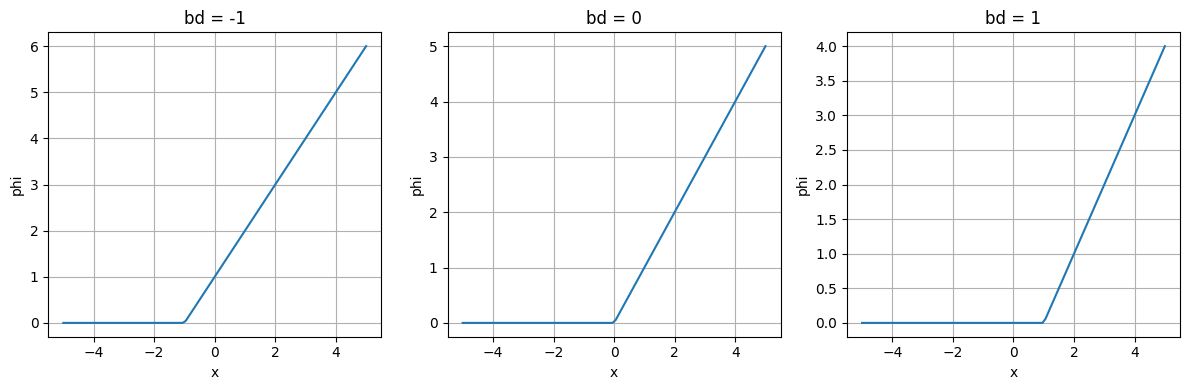
\includegraphics[width=1\textwidth]{src/random_relu.png}
        \caption{Tracé de la fonction $\phi(\cdot)$ pour différentes valeurs de $b_d$.}
        \label{fig:random_relu}
    \end{figure}

    \newpage

    Il s'agit d'une fonction d'activation ReLU.\\


    \item La fonction h est une fonction d'activation ReLU appliquée à une combinaison linéaire, c'est donc une fonction affine par morceaux.\\
    Les $w_k$ représentent les coefficients directeurs de toutes les droites affines qui permettront d'approximer la fonction recherchée.\\

    Il est nécessaire d'avoir un grand nombre de ces droites (nombre $D$) pour obtenir une approximation aussi précise que possible.\\

    \item On suppose que $x \in \mathbb{R}^P, P \in \mathbb{N}$ et que $\phi_d(x) = max(\langle x, v_d\rangle - b_d, 0)$, où $v_d$ vit sur la sphère unité.
    On a donc : $\phi_d(x) = max(\sum_{i=1}^P x_i v_{d,i} - b_d, 0)$\\
\end{enumerate}


\section{Mise en place sur PyTorch}

Dans ce TP, nous allons complètement nous affranchir de numpy.
C’est une librairie de calcul pratique et plutôt efficace.
Cependant, PyTorch offre des fonctionnalités similaires et plusieurs de ses fonctions sont mieux optimisées.
De plus, cette librairie permet de travailler sur GPU ou CPU sans effort.\\

Nous définissons aussi la fonction $f$ à apprendre sur l’intervalle $[-1, 1]$ :\\

\code{
    \# The function to learn\\
    def f(X):\\
    \indent \qquad return (torch.abs(X)*torch.sin(2*2*torch.pi*X)).type(dtype)
}

\subsection{Préliminaires}

\begin{enumerate}
    \item La figure \ref{fig:trace_f} présente le tracé de la fonction $f$.
    
    \begin{figure}[ht]
        \centering
        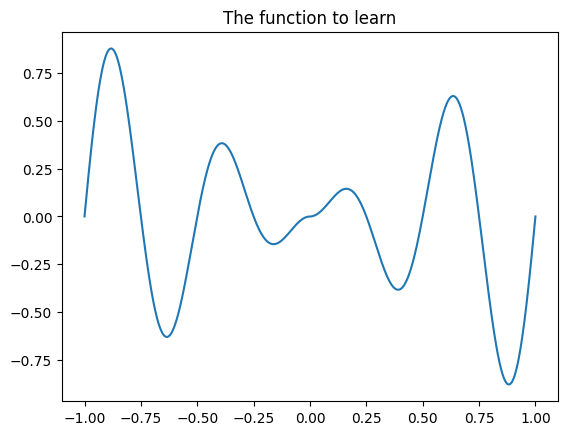
\includegraphics[width=0.5\textwidth]{src/trace_f.png}
        \caption{Tracé de la fonction $f$.}
        \label{fig:trace_f}
    \end{figure}


    \item On génère un jeu d'apprentissage $(x_n, y_n)$ en échantillonnant la fonction $f$ suivant les positions $x_n = -1 + \frac{2n}{N}$ où $N$ est le nombre total de mesures d’entraînement et $y_n = f(x_n)$.
    
    \code{
        \# Number of training samples\\
        N = 100\\

        \# Generate training data\\
        X\_train = torch.linspace(-1, 1, N).to(device)\\
        Y\_train = f(X\_train)
    }

    L’objectif ici va être d’approcher la fonction $f$ à partir des points d’échantillonnage $(x_n, y_n)$ :

    \begin{figure}[ht]
        \centering
        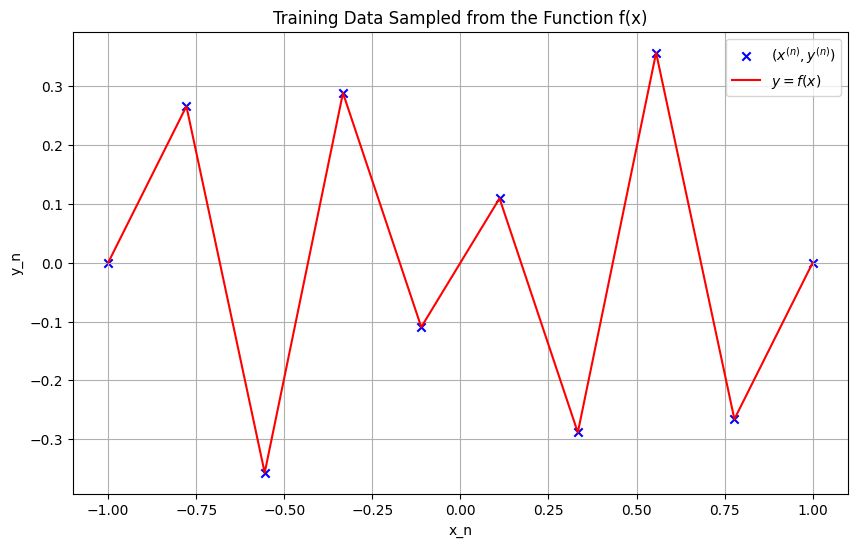
\includegraphics[width=0.5\textwidth]{src/trace_f_echantillonne.png}
        \caption{Tracé de la fonction $f$ échantillonnée.}
        \label{fig:trace_f_echantillonne}
    \end{figure}
    

    \end{enumerate}


Considérons le problème d’optimisation du risque empirique suivant :
\begin{equation}
    \underset{w \in \mathbb{R}^D}{\text{inf }} R_N(w) \quad \text{avec} \quad R_N(w) = \frac{1}{2N} \sum_{n=1}^N ||h(x_n, w) - y_n||^2_2
    \label{eq:R_N}
\end{equation}

\newpage

\subsection{Un peu de géométrie}

\begin{enumerate}
    \item On détermine une condition sur les coefficients $b_d$ pour qu’il existe un poids $w$ tel que $R_N(w) = 0$ :\\
    On remarque que la fonction $R_n(w)$ est forcement nulle en -1.
    Ainsi, pour pouvoir atteindre la premiere valeur du maillage, il faut qu'il existe un $b_d$ avant d'ou :
    $\exists b_d \text{ tel que }  b_d < x_0 $.\\
    Ensuite, pour atteindre chaque point il suffit d'avoir un $b_d$ entre chaque point du maillage.\\
    Ainsi, on a : $\forall i \in [1,n], \quad \exists b_d \text{ tel que }  b_d \in ]x{i-1},x_i[ $.
    



    \item On a : $\qquad h(x_n, w) = \sum_{d=1}^D w_d \phi_d(x_n)$.\\
    
    On pose : $\qquad \psi_n = (\phi_1(x_n), \dots, \phi_D(x_n))$\\

    On a donc : $\qquad h(x_n, w) = \langle w, \psi_n \rangle$\\

    On pose également : $\qquad Y = \begin{pmatrix}
        y_1 \\
        \vdots \\
        y_N
        \end{pmatrix} \in \mathbb{R}^N \quad$ et $\quad W = \begin{pmatrix}
        w_1 \\
        \vdots \\
        w_D
        \end{pmatrix} \in \mathbb{R}^D$.\\

    Soit $\qquad \Psi = \begin{pmatrix}
        \psi_1^T \\
        \vdots \\
        \psi_N^T
        \end{pmatrix} \in \mathbb{R}^{N \times D}$.\\

    On a donc : $\qquad R_N(w) = \frac{1}{2N} ||\Psi W - Y||_2^2$\\

    Le problème \eqref{eq:R_N} devient donc : $\qquad \underset{w \in \mathbb{R}^D}{\text{inf }} \frac{1}{2N} ||\Psi W - Y||_2^2$\\

    C'est un problème de moindres carrés : il est convexe et différentiable.
    La solution est unique si et seulement si $\Psi$ est de rang plein (ou $\Psi^T \Psi$ est inversible).\\
\end{enumerate}


\subsection{Opérations sur les tenseurs}
PyTorch permet de faire des opérations sur des tenseurs de taille différentes.
Nous avons donc mis en place des expériences en comprendre les méchanismes.

\begin{enumerate}
    \item On construit un tenseur $\texttt{A}$ de taille $3 \times 1$ et un tenseur $\texttt{B}$ de taille $1 \times 4$ :
    
    \code{
        A = torch.tensor([[1], [2], [3]])\\
        B = torch.tensor([[4, 5, 6, 7]])
    }

\newpage

    \item On calcule $\texttt{A + B}$ en PyTorch :
    
    \code{
        C = A + B\\
        print(C)\\
        \# tensor([[5, 6, 7, 8],\\
        \#         [6, 7, 8, 9],\\
        \#         [7, 8, 9, 10]])
    }

    L'opération effectuée ici est une addition terme à terme entre la matrice $\texttt{A}$ dont les lignes sont dupliquées et la matrice $\texttt{B}$ dont les colonnes sont dupliquées.
    
    \item On construit maintenant un tenseur $\texttt{A}$ de taille $3$ et un tenseur $\texttt{B}$ de taille $4$ et on calcule $\texttt{A[:, N one] + B[N one, :]}$ :
    
    \code{
        A = torch.tensor([1, 2, 3])\\
        B = torch.tensor([4, 5, 6, 7])\\
        C = A[:, None] + B[None, :]\\
        print(C)\\
        \# tensor([[5, 6, 7, 8],\\
        \#         [6, 7, 8, 9],\\
        \#         [7, 8, 9, 10]])
    }

    On obtient le même résultat qu'à la question précédente.

\end{enumerate}


\subsection{Le code principal}

\begin{enumerate}
    \item On construit une classe PyTorch définissant le modèle $h$.
    Elle prend la forme suivante :

    \code{
        class one\_layer\_NN(nn.Module):\\
        \indent\qquad def \_\_init\_\_(self, n\_hidden = 10):\\
        \indent\qquad \qquad super(one\_layer\_NN, self).\_\_init\_\_()\\
        \indent \qquad \qquad self.b = 2*(torch.rand(n\_hidden)-0.5).to(device)\\
        \indent \qquad \qquad self.w = torch.nn.Parameter(torch.zeros(n\_hidden))\\
        \indent \qquad def forward(self, x):\\
        \indent \qquad \qquad dif = x - self.b[None,None,:]\\
        \indent \qquad \qquad hidden = torch.maximum(dif,torch.zeros\_like(dif))\\
        \indent \qquad \qquad return torch.sum(self.w[None,None,:]*hidden, keepdim=True, dim=2)
    }

    \item En prenant exemple sur le TP2, nous avons codé un algorithme d’optimisation stochastique pour minimiser le risque empirique sous PyTorch.\\
    

\newpage

    \item On affiche la fonction $h(\cdot, w)$ toutes les $1000$ ainsi que son adéquation aux données sur la figure suivante :
    
    \begin{figure}[ht]
        \centering
        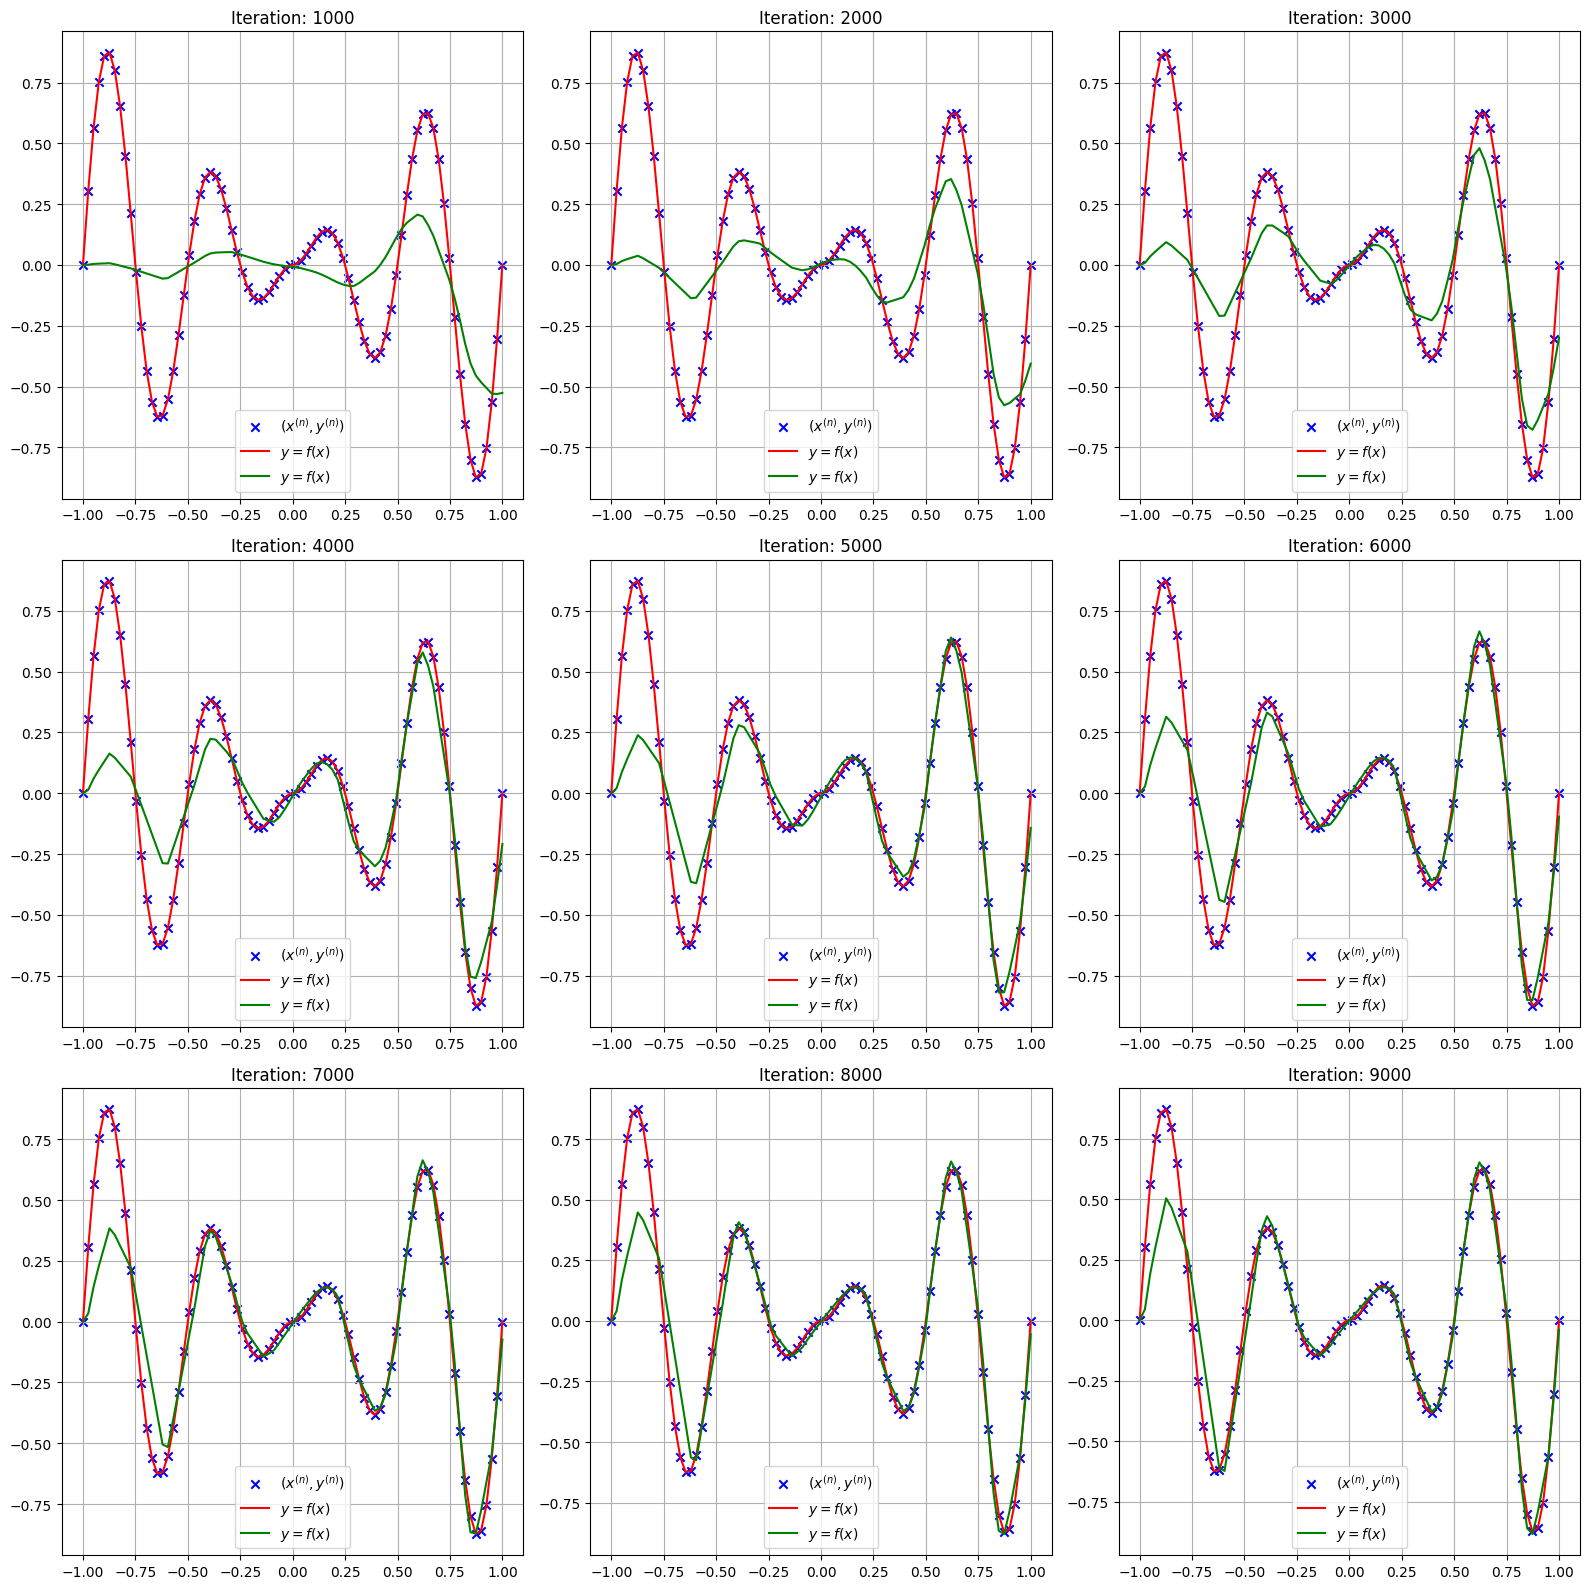
\includegraphics[width=1\textwidth]{src/h_w.png}
        \caption{Fonction $h(\cdot, w)$ et son adéquation aux données.}
        \label{fig:h_w}
    \end{figure}

    Après avoir effectué plusieurs tests d'optimiseurs (avec un nombre de points $N = 100$ et $D = 100$), on décide de garder l'optimiseur Adam de la librairie torch.optim avec un taux d'apprentissage : $lr = 10^{-3}$.\\
    La figure ci-dessus illustre l'apprentissage de la fonction au cours des itérations avec ces paramètres.

\end{enumerate}


\newpage

\section{Analyse des résultats}

\begin{enumerate}
    \item Pour $N = 10$, on obtient l'échantillonnage suivant :
    
    \begin{figure}[ht]
        \centering
        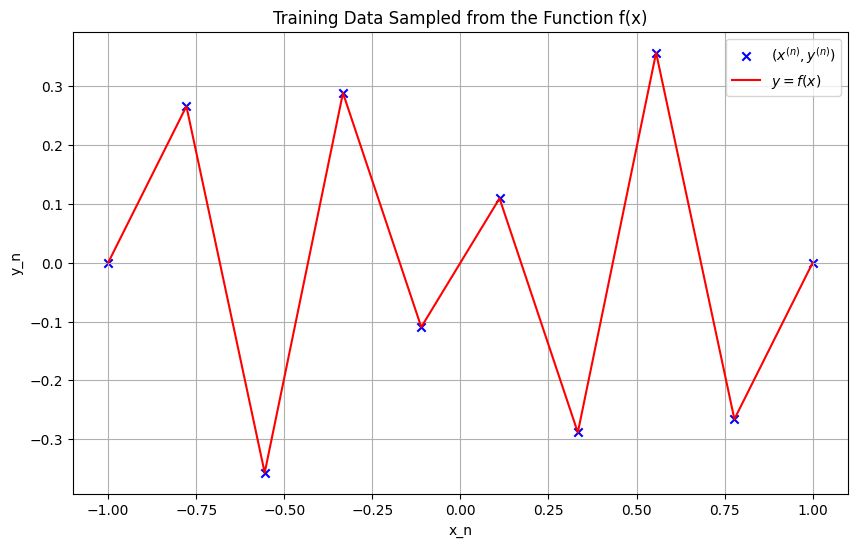
\includegraphics[width=0.5\textwidth]{src/trace_f_echantillonne.png}
        \caption{Tracé de la fonction $f$ échantillonnée avec $N = 10$.}
        \label{fig:trace_f_echantillonne10}
    \end{figure}
    


    \item On calcule la solution de \ref{eq:R_N} pour différentes valeurs de $D$.
    \begin{itemize}
        \item En régime sous-paramétré :
        \begin{figure}[ht]
            \centering
            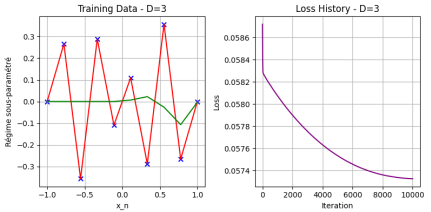
\includegraphics[width=0.5\textwidth]{src/P1.png}
            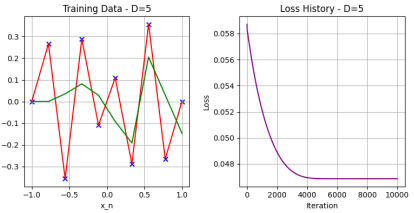
\includegraphics[width=0.5\textwidth]{src/P2.png}
            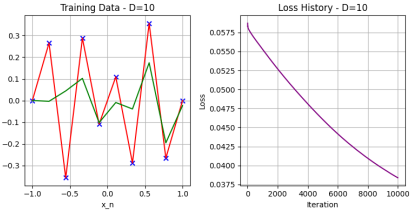
\includegraphics[width=0.5\textwidth]{src/P3.png}
            \caption{Solution en régime sous-paramétré.}
            \label{fig:regime_sous_parametre}
        \end{figure}

        Pour ce régime avec de faibles valeurs de D le résultats obtenu n'est pas très satisfaisant.
        La fonction verte qui est la fonction prédite est très loin de la fonction originale.
        De plus on voit sur l'historique de la fonction loss que ces 3 modèles ne vont pas converger, la fonction perte stagne autour d'une valeur égale à $10^{-2}$ .\\


        \item En régime limite :
        \begin{figure}[ht]
            \centering
            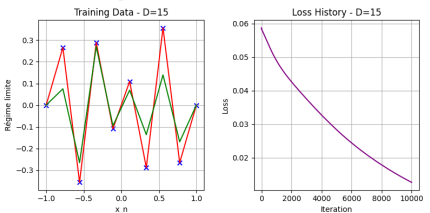
\includegraphics[width=0.5\textwidth]{src/P4.png}
            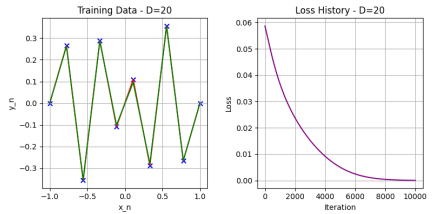
\includegraphics[width=0.5\textwidth]{src/P5.png}
            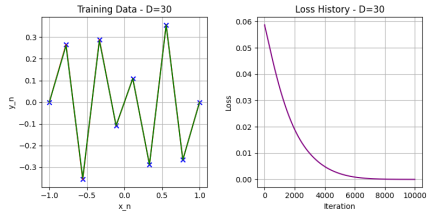
\includegraphics[width=0.5\textwidth]{src/P6.png}
            \caption{Solution en régime limite.}
            \label{fig:regime_limite}
        \end{figure}

        Les fonctions prédite des modèles en régime limite sont beaucoup plus proches de la fonction à estimer.
        A partir de $D = 20 $ la fonction est quasiment reproduite à l'identique avec des loss très faible de l'ordre de $10^{-5} $ .
        Selon la courbe de \ref{fig:courbe_reference} on voit que l'on a déjà atteint la valeur limite entre la sous-paramétrisation et la sur-paramétrisation.\\

        \newpage

        \item En régime sur-paramétré :
        \begin{figure}[ht]
            \centering
            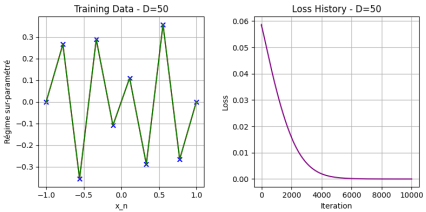
\includegraphics[width=0.5\textwidth]{src/P7.png}
            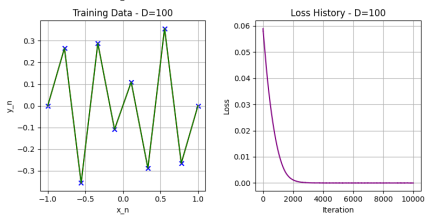
\includegraphics[width=0.5\textwidth]{src/P8.png}
            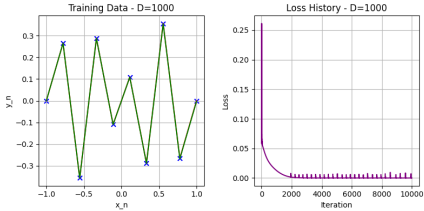
\includegraphics[width=0.5\textwidth]{src/P9.png}
            \caption{Solution en régime sur-paramétré.}
            \label{fig:regime_sur_parametre}
        \end{figure}

        Dans le régime surparamétré les 3 fonctions prédites se surperposent totalement à la fonction à estimer et on remarque que la fonction loss converge très rapidement vers 0.
        Mais un phénomène très bizarre apparaît, avec $D = 100$ on observe des pics dans la fonction loss qui sont des témoins purs de l'overfitting.\\

        
    \end{itemize}

    \newpage

    \item Nous allons essayer de quantifier cette observation.
    Pour ce faire, nous avons tracé le risque moyen pour différentes valeurs de $D$ à la figure \ref{fig:risque_moyen}.

    \begin{figure}[ht]
        \centering
        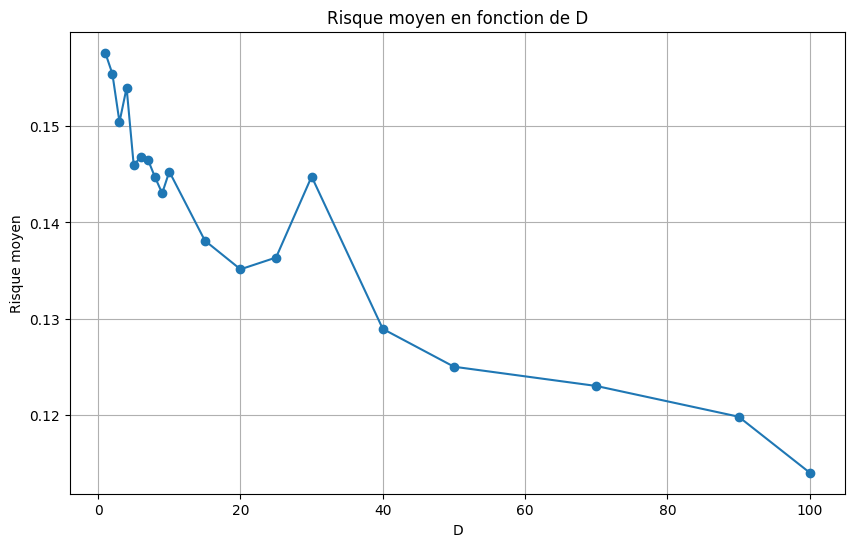
\includegraphics[width=0.5\textwidth]{src/risque_moyen.png}
        \caption{Risque moyen pour différentes valeurs de $D$.}
        \label{fig:risque_moyen}
    \end{figure}

    L'allure de la courbe est cohérente avec la courbe de référence :
    \begin{figure}[ht]
        \centering
        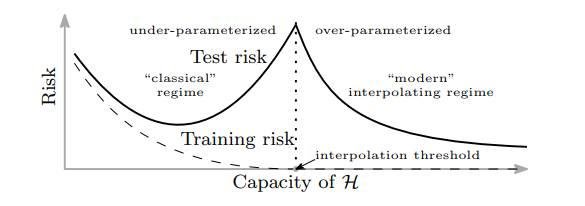
\includegraphics[width=0.5\textwidth]{src/courbe_reference.png}
        \caption{Courbe de référence.}
        \label{fig:courbe_reference}
    \end{figure}
\end{enumerate}




\section{Gradient stochastique et surparamétrisation}
Finalement, on se propose d’analyser empiriquement le comportement du gradient stochastique dans le régime surparamétré.
Da façon informelle, on a le résultat suivant :

\begin{tcolorbox}[colback=red!5!white,colframe=red!25!black]
    Dans un régime surparamétré, le gradient stochastique à pas constant converge, tandis qu’il ne converge pas sinon.
\end{tcolorbox}


La raison intuitive derrière cette propriété est que les gradients des fonctions individuelles $f_i$ s’annulent de façon synchrone sur les minimiseurs globaux.
C’est un peu comme s’il y avait une réduction de variance automatique.

\begin{enumerate}
    \item Nous avons lancé une descente de gradient stochastique avec un mini-batch pour $D = 5$ et $D = 1000$. De plus nous avons configurer l'algorithme de gradient stochastique avec un nombre de points N = 100 et un $batch\_size $ = 10.

    La figure \ref{fig:gradient_stochastique} présente le risque empirique à chaque itération pour ces deux valeurs de $D$.

    \begin{figure}[t]
        \centering
        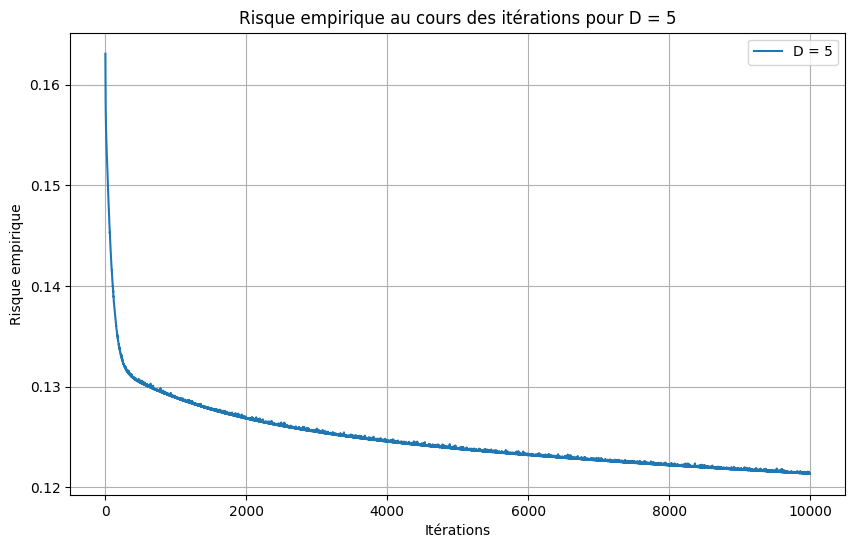
\includegraphics[width=7.3cm]{src/gradient_stochastique_5.png}
        \hfill
        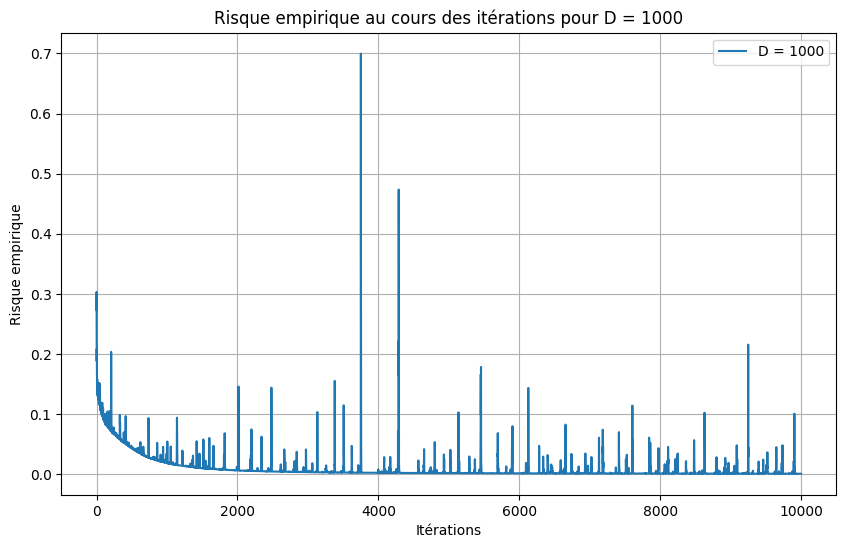
\includegraphics[width=7.3cm]{src/gradient_stochastique_1000.png}
        \caption{Risque empirique à chaque itération pour $D = 5$ et $D = 1000$.}
        \label{fig:gradient_stochastique}
    \end{figure}

    \newpage

    \item Est-ce que vous voyez une différence de comportement dans le régime sur-paramétré et dans le régime sous-paramétré ?

    On remarque sur ces 2 figures les différences entre les le régime sous-paramétré et le régime sur-paramétré. Le régime sous-paramétré à un très gros défaut, celui-ci n'arrive pas à converger, le risque empirique stagne même en augmentant le nombre d'itérations.
    Le régime sur-paramétré lui converge mais il y a un autre problème caractéristique de l'overfitting, il y a des énorme pics dans la fonctions loss ainsi en fonction de l'itération il peut donner un risque empirique totalement abberant.

\end{enumerate}


\end{document}